\documentclass[conference]{IEEEtran}
\IEEEoverridecommandlockouts
\usepackage[T1]{fontenc}
\usepackage[utf8]{inputenc}
\usepackage{cite,amsmath,amssymb,graphicx,booktabs,array,tabularx}
\usepackage{algorithm,algorithmic}
\usepackage{tikz,pgfplots}
\usepackage[hyphens]{url}
\usepackage{xurl}
\usepackage[hidelinks]{hyperref}
\usepackage{microtype}
\usetikzlibrary{arrows.meta,positioning,calc}
\pgfplotsset{compat=1.17}
\definecolor{inkblue}{RGB}{42,97,130}
\definecolor{mutedgreen}{RGB}{71,123,103}
\definecolor{mutedamber}{RGB}{173,124,52}
\definecolor{mutedred}{RGB}{153,77,82}
\newcolumntype{Y}{>{\raggedright\arraybackslash}X}
\newcommand{\sys}{GDN Tree-Scan}
\newcommand{\pending}[1]{\textit{Planned; results pending: #1.}}
% Generated from archived JSON.
\newcommand{\NativeFiveAccepted}{3.422}
\newcommand{\NativeFiveCommitted}{4.422}
\newcommand{\NativeFiveEventMs}{103.45}
\newcommand{\NativeFiveTPS}{42.74}
\newcommand{\NativeFiveOccupancy}{2.79}
\newcommand{\NativeElevenAccepted}{4.923}
\newcommand{\NativeElevenCommitted}{5.923}
\newcommand{\NativeElevenEventMs}{148.28}
\newcommand{\NativeElevenTPS}{39.95}
\newcommand{\NativeElevenOccupancy}{2.74}
\newcommand{\TreeAccepted}{4.286}
\newcommand{\TreeCommitted}{5.286}
\newcommand{\TreeEventMs}{160.88}
\newcommand{\TreeTPS}{32.85}
\newcommand{\TreeOccupancy}{2.80}
\newcommand{\BreakEvenAccepted}{5.88}
\newcommand{\BreakEvenEventMs}{123.66}
\newcommand{\RequiredReduction}{23.1}

\begin{document}
\title{GDN Tree-Scan: Correct State Commitment and Performance Limits of Tree Speculation in Recurrent Hybrids}
\author{\IEEEauthorblockN{Zhiyuan Ma}
\IEEEauthorblockA{\texttt{zhiyuanma0520@gmail.com}}
\thanks{Working revision, September 22, 2026. Archived witnesses, fresh arithmetic diagnostics, and current-stack timing are identified separately.}}
\maketitle
\begin{abstract}
Tree speculative decoding for recurrent-hybrid language models must preserve candidate ancestry and continuation state. We study GDN Tree-Scan, a Gated DeltaNet verifier whose accepted-prefix contract coordinates recurrent state, convolution history, attention storage, and pending correction tokens. Archived regression witnesses expose incomplete state publication and physical-layout-dependent numerical disagreement. The publication repair changes one token fixture from 15 failures in 15 checks to zero. Fresh same-input measurements compare sequential scan/replay with local triangular-solve and finite-Neumann reconstructions on eight pilot prefixes and 31 of 32 confirmation prefixes passing frozen provenance checks. Frozen numerical, padding, and timing criteria fail, preventing promotion of the compact routes; a retrospective audit also identifies omitted checks and inaccurate pilot rationale. After bounded state, greedy-path, and output checks, eighteen fresh boots on GB10 compare three instrumented Qwen3.6-27B-FP8 configurations. Against native five-step multi-token prediction, the tree averages 12.69 versus 13.67 tokens/s at batch one and 47.28 versus 55.38 at batch four; it exceeds the longer eleven-step control. These rates bind returned tokens to the same physical wall intervals. Engine seeds differ across arms, and only 14 of 144 same-block, across-arm prompt-stream comparisons are exactly equal. The results therefore describe the configurations as executed, with coarse three-block uncertainty. They provide scoped state-integrity witnesses and numerical/cost characterization, without establishing full-model sequential equivalence, quality preservation, or an isolated tree-algorithm speedup.
\end{abstract}

\begin{IEEEkeywords}
speculative decoding, Gated DeltaNet, state commitment, numerical reproducibility, language-model serving
\end{IEEEkeywords}

\section{Introduction}
Speculative decoding reduces serial target-model invocations by verifying draft tokens in parallel. Its sampling guarantee assumes that verification supplies the intended target probabilities. Tree speculation expands the candidate set, but it does not relax that assumption~\cite{leviathan2023fast,chen2023sampling,miao2023specinfer}. For recurrent-hybrid models, realizing the verifier requires more than an attention mask: a candidate must inherit the state of its ancestors, and the next serving iteration must inherit exactly the path selected for continuation~\cite{yang2024gated,wu2025stree}.

This paper studies that boundary in \sys{}, a Gated DeltaNet verifier integrated with vLLM and a fork of FlashAttention-2. The implementation uses branch-local recurrent computation, device-side multidraft selection, and accepted-path publication across recurrent state, convolution history, and attention key--value (KV) storage~\cite{lumo2026receipts,lumo2026stateless}. An attention-KV mapping error demonstrates why repairing only the recurrent state is insufficient: a valid selected token path can still read a rejected sibling on the next iteration. A second failure arises even when masked branches contribute zero attention weight. Moving the visible spine keys changes floating-point reduction association and can alter a near-tied verification decision~\cite{lumo2026spine}.

Acceptance length also leaves the performance question incomplete. In one archived campaign configured for batch four, accepted drafts plus one per event averaged 5.286 for the tree and 4.422 for native five-step multi-token prediction. The archived rate proxy was lower for the tree: 32.85 versus 42.74 structural tokens/s~\cite{lumo2026cost,lumo2026archive}. This proxy divides the global accepted-plus-one mean by a mean cost drawn from a different, pure-decode event population; it is not a directly measured emitted-token throughput. The support mismatch motivates matched accounting for output, wall time, and component costs in current-system measurements.

\begin{figure}[t]
\centering
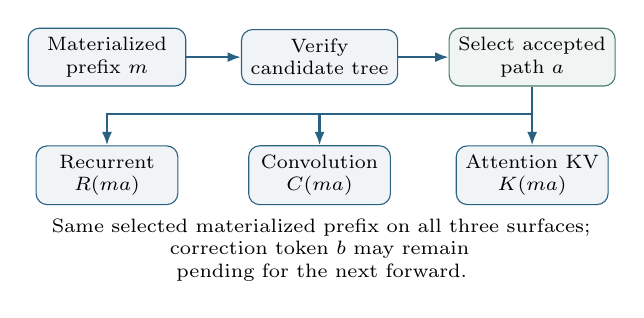
\begin{tikzpicture}[font=\scriptsize,
 box/.style={draw=inkblue,fill=inkblue!7,rounded corners,align=center,minimum height=0.7cm},
 arr/.style={-{Latex[length=1.7mm]},thick,draw=inkblue}]
\node[box,minimum width=2.0cm] (prefix) at (0,0) {Materialized\\prefix $m$};
\node[box,minimum width=1.8cm] (tree) at (2.7,0) {Verify\\candidate tree};
\node[box,draw=mutedgreen,fill=mutedgreen!8,minimum width=2.0cm] (path) at (5.4,0) {Select accepted\\path $a$};
\draw[arr] (prefix)--(tree);\draw[arr] (tree)--(path);
\node[box,minimum width=1.8cm] (r) at (0,-1.5) {Recurrent\\$R(ma)$};
\node[box,minimum width=1.8cm] (c) at (2.7,-1.5) {Convolution\\$C(ma)$};
\node[box,minimum width=1.8cm] (k) at (5.4,-1.5) {Attention KV\\$K(ma)$};
\draw[arr] (path.south) -- ++(0,-0.35) -| (r.north);
\draw[arr] (path.south) -- ++(0,-0.35) -| (c.north);
\draw[arr] (path.south)--(k.north);
\node[align=center,text width=7cm] at (2.7,-2.45) {Same selected materialized prefix on all three surfaces;\\correction token $b$ may remain pending for the next forward.};
\end{tikzpicture}

\caption{A selected token path must have a matching continuation state. Recurrent, convolution, and attention-KV state must all describe the same materialized prefix. A newly sampled token can remain pending until the next forward, just as in native decoding.}
\label{fig:contract}
\end{figure}

The revision makes four bounded contributions. First, it states the accepted-prefix contract at the actual serving boundary and associates it with concrete regression witnesses. Second, it explains a physical-layout source of numerical spine disagreement and the tested repair. Third, it reconciles archived acceptance and timing results and binds emitted tokens to physical wall intervals in eighteen fresh current-stack boots. These measurements compare the tree with depth-comparable five-step and longer eleven-step chains, with observed output divergence and an engine-seed deviation disclosed. The archive also includes a separate paired attention-kernel improvement. That optimization reduced its tested batch-four step time by 27.03\,ms, but does not establish tree-over-chain superiority~\cite{lumo2026paired}. Fourth, a fresh same-input kernel study characterizes scan, triangular-solve, and finite-Neumann arithmetic against distinct native references, including failed frozen criteria and an audit of omitted checks.

Parallel GDN tree verification and compact accepted-state reconstruction are already addressed by direct related work. Section~\ref{sec:related} positions this study accordingly. We do not claim a first hybrid-tree system, general bitwise equivalence, or a measured advantage over those implementations. Section~\ref{sec:planned} separates the completed bounded evidence from tests needed for stronger claims.

\section{Background and Related Work}
\label{sec:related}
\subsection{Drafting, verification, and serving}
Speculative sampling constructs an exact target sample from proposal and residual distributions, conditional on the probabilities actually supplied~\cite{leviathan2023fast,chen2023sampling}. SpecInfer supplies the tree-verification framing; Sequoia, EAGLE-2, and OPT-Tree investigate tree construction and its performance consequences~\cite{miao2023specinfer,chen2024sequoia,li2024eagle,wang2024opt}. Our study keeps these algorithmic questions separate from whether a deployed kernel and cache return the intended probabilities.

PagedAttention and SGLang address the scheduling, memory, and execution substrate~\cite{kwon2023efficient,zheng2024sglang}. Hybrid serving additionally manages recurrent-state pools alongside KV storage, as documented by SGLang's hybrid-model integration~\cite{pytorch2025sglang,sglang2026qwen}. Thus neither a fast isolated recurrent kernel nor low transient state memory alone determines user-visible latency. FlashAttention-2's work partitioning supplies the attention substrate examined here~\cite{dao2023flashattention}.

\subsection{Recurrent and hybrid speculation}
Gated DeltaNet augments a decayed recurrent state with a data-dependent delta update~\cite{yang2024gated}. Parallel delta-rule formulations provide relevant algebraic background~\cite{yang2024delta}. Stateful speculation is established territory: STree studies speculative trees for hybrid state-space models, SpecMamba targets an FPGA implementation, and component-aware self-speculation studies how hybrid components affect the design~\cite{wu2025stree,zhong2025specmamba,borobia2026component}. These works motivate an explicit state lineage; they do not justify treating every recurrent update or numerical implementation as interchangeable.

\subsection{Direct GDN comparisons}
\textbf{Bole} derives a tree-structured closed form and evaluates it with a value-tiled finite-polynomial solver. It stores compact update factors and reconstructs the accepted state. Its SGLang integration combines batch-wide verification budgeting with captured GPU execution. Evaluation includes unquantized Qwen3.5-27B on GB10 and online replay of agent sessions~\cite{wang2026bole}. Its state and serving mechanisms directly overlap the problem studied here. Our measured replay cost is therefore not a lower bound on alternative implementations.

Concretely, Bole's correction system is $(I+G)U=R$, where $G$ contains strict-ancestor interactions and $R$ is the source correction. Tree depth $d$ gives $G^{d+1}=0$, so $U=\sum_{m=0}^{d}(-G)^mR$. This finite identity changes the arithmetic schedule from sequential updates to matrix propagation~\cite{wang2026bole}. Our path preserves sequential updates and replays accepted operands; Section~\ref{sec:reconstruction-numerics} explains why the numerical comparison remains an empirical question.

\textbf{TreeWY} expresses GDN tree verification as a triangular system and reconstructs the accepted state from pseudo-values. Its vLLM evaluation uses Qwen3.5-35B and 397B on B200, greedy verification, and disabled prefix caching. It explicitly permits finite-precision disagreement with the baseline and reports that wider trees improve acceptance without yet winning throughput~\cite{ghantasala2026treewy}. Consequently, shared-spine byte checks in our particular route neither establish that TreeWY is incorrect nor replace its serving comparison.

\textbf{ReplaySSM} caches recurrent inputs and changes when state is materialized; its implementation RFC includes GDN and Mamba2~\cite{replayssm2026}. Reconstruction and replay are not claimed as new concepts here. Table~\ref{tab:related} states the comparison boundary. Published speed ratios from different checkpoints, precision formats, workloads, and software builds are not combined into a performance ranking.

\begin{table}[t]
\caption{Direct comparison scope. External methods were read, not executed in this revision.}
\label{tab:related}
\centering\footnotesize
\begin{tabularx}{\columnwidth}{@{}>{\raggedright\arraybackslash}p{0.22\columnwidth}YY@{}}
\toprule
Method & Overlapping mechanism & Boundary for this study \\
\midrule
Bole~\cite{wang2026bole} & Parallel verifier; factorized commit & Different stack and precision; no matched run \\
TreeWY~\cite{ghantasala2026treewy} & Tree solve; accepted-state reconstruction & Different models and operating regime; no matched run \\
ReplaySSM~\cite{replayssm2026} & Input caching; deferred state work & Alternative state policy; no matched run \\
\sys{} & Scan/replay; accepted-path remapping & Specific numerical and lifecycle witnesses; scoped cost evidence \\
\bottomrule
\end{tabularx}
\end{table}

\section{The Accepted-Prefix Contract}
\label{sec:contract}
\subsection{State and the execution boundary}
Let $m$ be a materialized token prefix: the tokens already consumed by the target's forward computation. Write its persistent state as
\begin{equation}
\mathcal{S}(m)=\bigl(R(m),C(m),K(m)\bigr),
\end{equation}
where $R$ collects recurrent matrices, $C$ collects convolution histories, and $K$ collects attention KV entries. The logical emitted prefix can also include a newly sampled token $b$ that has not yet been consumed. The continuation boundary is then $(\mathcal{S}(m),b)$, not a claim that $\mathcal{S}(mb)$ has already been computed. This distinction is essential when counting the correction or bonus token while checking cache state.

A tree descriptor contains candidate token IDs, parent indices, depth/position information, attention visibility, and maps between logical nodes and physical slots. For a candidate node $i$, each target layer must consume the state obtained from the candidate's root-to-parent path. At publication, the selected materialized path, pending-token convention, and next-drafter input row must agree. Figure~\ref{fig:contract} illustrates the three state surfaces documented by the implementation audit~\cite{lumo2026stateless,lumo2026archive}.

\subsection{The recurrence and path locality}
For one GDN head, let $R\in\mathbb{R}^{d_v\times d_k}$. Queries and keys are in $\mathbb{R}^{d_k}$ and values in $\mathbb{R}^{d_v}$. With decay $\alpha_i$ and write strength $\beta_i$, a node applies the standard update~\cite{yang2024gated}
\begin{align}
R'_i &= \alpha_i R_{\pi(i)}, &
\delta_i &= \beta_i\bigl(v_i-R'_i k_i\bigr),\\
R_i &= R'_i+\delta_i k_i^\top, &
o_i &= R_iq_i,
\end{align}
where $\pi(i)$ is its parent. A previous node in the packed buffer need not be $\pi(i)$. The causal convolution likewise requires path predecessors rather than adjacent packed rows. The attention visibility relation must select the same logical prefix and ancestry. These requirements follow from the model's computation; a correct attention mask cannot repair a wrong recurrent parent.

The implementation verifies nodes with branch-local scratch and makes the selected continuation durable through replay and remapping. This is an implementation route, not the only way to satisfy the contract~\cite{lumo2026receipts,lumo2026stateless}. In particular, rejecting a branch requires that its contents cannot influence future computation; it does not require zeroing every scratch byte if future reads are correctly restricted.

\subsection{Four different correctness questions}
\textit{Algebraic correctness} asks whether the recurrence or its reformulation computes the same real-arithmetic function. \textit{Numerical agreement} asks whether particular kernels, layouts, and precisions agree with a selected reference. \textit{Sampler correctness} asks whether the acceptance/residual rule returns its supplied target distribution. \textit{Serving correctness} asks whether these properties survive cache restoration, row reuse, batching, and the next iteration~\cite{yang2024delta,chen2023sampling,lumo2026archive}.

For example, for target probabilities $p$ and proposal probabilities $q$, accepted mass is $\min(p,q)$ under ordinary rejection sampling. Sampling the remaining mass proportional to $(p-q)_+$ gives the target marginal. The argument is conditional on the actual proposal law and target probabilities; substituting stale logits or an incorrect state changes the distribution being sampled~\cite{leviathan2023fast,chen2023sampling}. The same distinction applies to the multidraft reference used here~\cite{miao2023specinfer,lumo2026receipts}.

If every iteration supplies the reference conditional probabilities and publishes an equivalent continuation boundary, an induction over emitted tokens gives the reference joint distribution. This is a conditional argument, not a proof that the implemented system satisfies its premises. A tolerance test, zero observed garble, or equal task outcomes does not discharge all those premises.

\section{Implementation and Failure Mechanisms}
\subsection{A descriptor shared by verification and commitment}
Figure~\ref{fig:pipeline} shows the served path. Native multi-token prediction (MTP) supplies the principal draft chain; selected variants add runner-up candidates. The descriptor maps each candidate through the attention mask, recurrent scan, sampler, and selected-path publication. Historical variants also use a heuristic suffix predictor; this changes the proposal source and must be recorded separately from tree topology~\cite{lumo2026receipts,lumo2026cost}.

\begin{figure}[t]
\centering
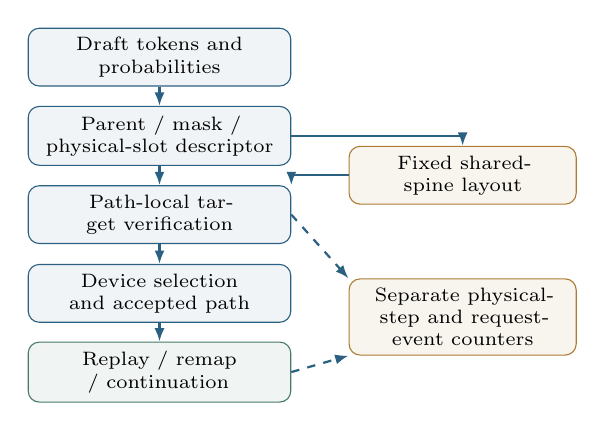
\begin{tikzpicture}[font=\scriptsize,
 box/.style={draw=inkblue,fill=inkblue!7,rounded corners,align=center,text width=3.1cm,minimum height=0.65cm},
 arr/.style={-{Latex[length=1.7mm]},thick,draw=inkblue}]
\node[box] (draft) at (0,0) {Draft tokens and probabilities};
\node[box] (desc) at (0,-1.0) {Parent / mask / physical-slot descriptor};
\node[box] (verify) at (0,-2.0) {Path-local target verification};
\node[box] (select) at (0,-3.0) {Device selection and accepted path};
\node[box,draw=mutedgreen,fill=mutedgreen!8] (commit) at (0,-4.0) {Replay / remap / continuation};
\foreach \a/\b in {draft/desc,desc/verify,verify/select,select/commit} \draw[arr] (\a)--(\b);
\node[box,text width=2.65cm,draw=mutedamber,fill=mutedamber!8] (spine) at (3.85,-1.5) {Fixed shared-spine layout};
\node[box,text width=2.65cm,draw=mutedamber,fill=mutedamber!8] (metrics) at (3.85,-3.3) {Separate physical-step and request-event counters};
\draw[arr] (desc.east) -| (spine.north);
\draw[arr] (spine.west) -| (verify.north east);
\draw[arr,dashed] (verify.east) -- (metrics.north west);
\draw[arr,dashed] (commit.east) -- (metrics.south west);
\end{tikzpicture}

\caption{One descriptor connects the target forward and the continuation state. The selected row also controls the next drafter input. Timing records must identify whether they count a physical step or a request verification event.}
\label{fig:pipeline}
\end{figure}

The attention fork applies an additive ancestry bias to speculative suffix scores while leaving the context visible. It retains the native prefill route. Recurrent nodes obtain their parent state from the pre-tree state or node-local scratch. After device selection, accepted-path replay and remapping establish the continuation state~\cite{lumo2026receipts}. Cache checkpoints and restored rows must obey the same contract; a correct cold first request does not establish correctness after a checkpoint hit or page reuse~\cite{lumo2026stateless}.

\begin{algorithm}[t]
\caption{Logical verifier and continuation boundary}
\label{alg:verify}
\begin{algorithmic}[1]
\REQUIRE Reference-aligned state boundary, candidate descriptor $T$
\STATE Map logical candidates to physical slots and positions.
\STATE Verify using path-local convolution, GDN, and attention.
\STATE Apply the configured sampler to matching target/proposal rows.
\STATE Obtain the accepted path and any pending correction token.
\STATE Publish recurrent and convolution state for the materialized path.
\STATE Map its attention KV entries to the native continuation layout.
\STATE Map the selected hidden-state row to the next drafter input.
\STATE Preserve the native pending-token and position convention.
\RETURN Continuation boundary and emitted-token accounting
\end{algorithmic}
\end{algorithm}

\subsection{Accepted state with the wrong attention KV}
The archived remap failure left recurrent and convolution state aligned with the selected path, while attention read a neighboring sibling's KV entry after a non-contiguous path was accepted~\cite{lumo2026stateless}. The fix copies each selected node's KV entry from its verification slot into its linear continuation slot. Its role is state movement rather than a new attention equation. Algorithm~\ref{alg:verify} makes the missing step explicit.

The associated token fixture changed from 15/15 failures to 0/15 across the reported eager, graph, and cold-cache checks. In served-script checks, the repaired cat8 and cat6 arms had zero observed corrupted-identifier flags among 84 and 61 scripts respectively~\cite{lumo2026stateless}. The pre-fix observations came from earlier runs, so their rates should not be treated as a randomized estimate of the repair's effect. The fixture supplies the more direct causal witness.

A later launcher audit found that previously validated remap and reorder flags were enabled in narrow launchers but disabled in the general campaign launcher. The corrected campaign therefore records post-boot engagement, not merely source-code availability~\cite{lumo2026archive}. This is why the identity of a compiled implementation and the effective configuration belong to the evidence boundary.

\subsection{Masked branches can change the shared spine}
In exact arithmetic, adding masked keys contributes zero to attention. In the tested FlashAttention-2 route, however, physical score columns also determine the association of the online-softmax reduction~\cite{dao2023flashattention,lumo2026spine}. Interleaving extra branch slots changes the positions of surviving spine keys. The visible values are unchanged, but their partial sums need not be associated identically.

\begin{figure}[t]
\centering
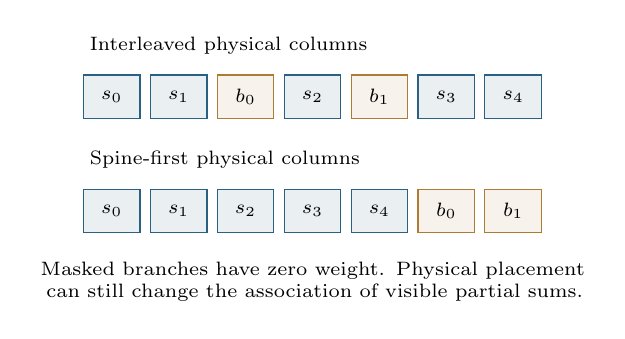
\begin{tikzpicture}[font=\scriptsize]
\node[anchor=west] at (-0.4,0.65) {Interleaved physical columns};
\foreach \i/\lab/\col in {0/s_0/inkblue,1/s_1/inkblue,2/b_0/mutedamber,3/s_2/inkblue,4/b_1/mutedamber,5/s_3/inkblue,6/s_4/inkblue}{
\node[draw=\col,fill=\col!10,minimum width=0.72cm,minimum height=0.55cm] at (\i*0.85,0) {$\lab$};}
\node[anchor=west] at (-0.4,-0.8) {Spine-first physical columns};
\foreach \i/\lab/\col in {0/s_0/inkblue,1/s_1/inkblue,2/s_2/inkblue,3/s_3/inkblue,4/s_4/inkblue,5/b_0/mutedamber,6/b_1/mutedamber}{
\node[draw=\col,fill=\col!10,minimum width=0.72cm,minimum height=0.55cm] at (\i*0.85,-1.45) {$\lab$};}
\node[align=center,text width=7cm] at (2.55,-2.35) {Masked branches have zero weight. Physical placement\\can still change the association of visible partial sums.};
\end{tikzpicture}

\caption{Illustrative physical slot layouts for one spine query. Blue entries are visible spine keys and amber entries are masked branches. The repair keeps shared-spine positions fixed within the tested execution layout. The drawing is a mechanism illustration, not a new numerical measurement.}
\label{fig:layout}
\end{figure}

The recorded witness shows a one-unit-in-the-last-place discrepancy in a bfloat16 output at magnitude eight: $2^{3-7}=0.0625$. The diagnostic identifies the shared attention spine and reports a greedy acceptance difference of 0.087 drafts/event between the compared tree variants~\cite{lumo2026spine}. Independent stochastic task traces cannot establish the same claim. A meaningful superset check fixes the common prefix, proposals, target reference, and decision rule. Under greedy longest-matching-path selection with unchanged shared-node outputs, adding candidates cannot remove an existing matching path. A numerical change can violate that premise.

The repair places the shared spine contiguously before other tree slots and propagates the permutation through the relevant maps. In the recorded observation harness and in-process check, the reordered shared spine matched the spine-only reference byte-for-byte; an interleaved control retained the discrepancy~\cite{lumo2026spine}. This is evidence for the tested route and shape family. Different compiler choices, kernel buckets, quantization formats, or sampling operations require their own checks. A fixed layout alone is not a universal floating-point identity theorem.

\subsection{Reconstruction, rounding, and accumulated disagreement}
\label{sec:reconstruction-numerics}
The archive includes an earlier local WY prototype. Its investigation reports a recurrent-state error of approximately $1.66\times10^{-3}$ and a subsequent maximum logit discrepancy of 3.32. The diagnosed state-write path reused an excessively rounded output representation. A separate state calculation reduced the isolated error; later assessments retained the algebraic equivalence and left broader acceptance-based validation open~\cite{lumo2026archive}. These are documentary observations about our historical prototype, not a reproduction or refutation of TreeWY. The evidence manifest identifies both the failure record and its later correction.

Other archived layer-localization studies examined our sequential tree route as well. They motivate a distinction between a local numerical discrepancy and its effect after further model layers or recurrent steps. A first-order explanatory model is $e_{\ell+1}\approx J_\ell e_\ell+\delta_\ell$: later layers can amplify an existing residual while introducing additional error. This expression is not a fitted error bound. Small local errors, or matching current outputs, do not establish matching future logits~\cite{lumo2026archive}.

The numerical reference must also be named. The pinned native speculative-update and one-token decode paths differ in gate rounding and state-storage boundaries. Our scan and replay share a sequential update body, but their compiled agreement still requires GPU checks~\cite{lumo2026archive}. Thus a real-arithmetic reconstruction identity does not by itself establish deployment agreement; conversely, disagreement with our selected reference does not establish an algebraic defect. E7a and E7b isolate verification arithmetic, state commitment, and subsequent continuation before measuring any deployment benefit. The E7a kernel-level pilot (Section~\ref{sec:e7a-pilot}) measures the first two of these boundaries: the two pinned native paths differ from each other by $2.2\times10^{-4}$ to $1.7\times10^{-3}$ of the state maximum on the tested operands, and an isolated ablation shows the difference is the decode kernel's documented bfloat16 rounding of the write gate (an oracle applying only that rounding matches it at the fp32 floor).

\section{Evaluation Protocol and Evidence Status}
\label{sec:protocol}
\subsection{Campaigns are separate experimental objects}
The main empirical material concerns Qwen3.6-27B-FP8 on GB10/DGX Spark~\cite{qwen2026qwen36fp8,lumo2026archive}. Table~\ref{tab:evidence} distinguishes the archived campaigns. They use different implementation stages and, in some cases, different harnesses. They are not replicates of a single final system. The accompanying evidence manifest records file paths and SHA-256 hashes; the accounting script recomputes the H3 table from stored JSON without running inference.

\begin{table*}[t]
\caption{Evidence carried into this draft. ``Verified archive'' means the reported observation was checked against an available source; it does not mean the experiment was rerun on the current code. P0, E7a, bounded E7b diagnostics, selected-route E2 checks, and eighteen E1 timing cells are executed. E3 remains conditional and E7c deferred.}
\label{tab:evidence}
\centering\footnotesize
\begin{tabularx}{\textwidth}{@{}p{0.05\textwidth}p{0.17\textwidth}Yp{0.25\textwidth}@{}}
\toprule
ID & Evidence & Supported statement & Important boundary \\
\midrule
H1 & KV-remap report~\cite{lumo2026stateless} & Fixture repair and observed post-fix script checks & Not a distribution proof or a randomized quality comparison \\
H2 & Spine-layout report~\cite{lumo2026spine} & Numerical witness, shared-spine repair, later acceptance values & Byte agreement scoped to tested reference and route \\
H3 & Postfix3 JSON and closeout~\cite{lumo2026archive} & Three-arm acceptance and mixed-population rate proxy & Historical nominal-B4 campaign; unmatched event populations and duplicated constraints \\
H4 & Paired attention optimization~\cite{lumo2026paired} & 27.03 ms local step reduction in its configuration & Different stage from H3; not a composed tree-over-chain result \\
H5 & Repeated-task audit~\cite{lumo2026archive} & Limits of the 16-task quality sample & Same Astropy subset; heterogeneous historical arms \\
H6 & Archived numerical investigations & Failure mechanism and later correction & Documentary evidence; original captures not reproduced \\
P0 & Configuration audit (Section~\ref{sec:protocol}) & Sampling reconstruction; no new model measurements & Historical binary gaps retained \\
E7a & Same-input kernel study (Section~\ref{sec:e7a-pilot}) & Historical/synthetic controls, eight fresh pilot prefixes, and 31 of 32 confirmation prefixes passing the frozen provenance checks & Local realizations, not the authors' systems; frozen numerical/control criteria missed; no model-level qualification \\
E2/E7b & Stage-isolated and selected-route checks (Sections~\ref{sec:e7b-diagnostic}--\ref{sec:selected-route}) & One-prefix propagation diagnostics and bounded B1/B4 serving-contract evidence & No live conv/KV byte snapshots, full-model sequential-equivalence or general sampler-law proof \\
E1 & Eighteen fresh timing boots (Section~\ref{sec:e1-timing}) & Three configurations, B1/B4, three paired blocks; exact token/wall support & Different continuations and engine seeds; coarse uncertainty; as-executed comparison \\
E3 & Conditional; not promoted & --- & No composed optimization result \\
\bottomrule
\end{tabularx}
\end{table*}

The H3 campaign configures four concurrent requests, enables prefix caching, and runs a 16-task Astropy subset drawn from SWE-bench Verified through qwen-code. Native MTP-5 uses five draft steps. MTP-11 matches the maximum draft depth of the tail6 tree, whose later suffix uses a different proposal source~\cite{lumo2026cost,lumo2026archive}. It is a useful strong control, but not a pure topology ablation. Task resolution follows the benchmark evaluation; the small chosen subset does not represent the full benchmark~\cite{jimenez2024swe}.

\subsection{Sampling provenance remains an explicit limitation}
Historical reports label several campaigns with requested temperature 0.6. The archive documents duplicated sampling constraints~\cite{lumo2026levers}. P0 reconstructs the three July patchers at their recorded, distinct source revisions against the launchers' pinned image: each produces two target-logit constraint calls, while the selected current revision produces one. This is source reconstruction, not recovery of the original patched runtime. The target-row temperature divisors compound to 0.36, but top-k/top-p filtering also repeats and bonus paths differ; the run is not equivalent to uniform temperature-0.36 sampling. We retain the requested settings as \emph{nominal}. Historical loaded-extension and model-file identities remain unresolved; current file hashes cannot establish July identity. The artifact includes the source reconstructions and per-arm audit manifests.

The stored numbers remain observations of the archived runs, useful for describing behavior and diagnosing cost. They do not provide a controlled-temperature estimate of the final system's advantage. Likewise, an available correctness test counts as a current passing result only when its execution record establishes the relevant route~\cite{lumo2026archive}.

\subsection{Tokens, events, physical steps, and service time}
Let $a_e$ be accepted drafts and $c_e$ be actual emitted tokens in request verification event $e$. For ordinary nonterminal events, $c_e=a_e+1$ because of a correction/bonus token. End-of-sequence and truncation instead require the actual count. A physical GPU step can contain several request events. A measured decode rate requires output counts and wall intervals from the same event population; component attribution also requires matching the timed operations to those events.

H3's archived instrument does not supply that matching. With $A_{\rm all}$ the global accepted-draft count, $D_{\rm all}$ the global draft-event count, $W_{\rm pure}$ retained pure-decode wall seconds, and $D_{\rm wall}$ their event count, its reported quantity is the accounting proxy
\begin{equation}
R_{\mathrm{H3\ proxy}}=
\frac{A_{\rm all}/D_{\rm all}+1}{W_{\rm pure}/D_{\rm wall}}.
\label{eq:rate}
\end{equation}
The wall instrument retains start-to-start intervals between consecutive pure-decode steps, caps idle intervals, and breaks the chain on mixed or prefill steps. Retained wall events cover only 74.19\%, 60.80\%, and 63.30\% of global draft events for MTP-5, MTP-11, and the tree. Accepted-token totals for that retained subset are absent. Moreover, accepted tokens plus draft events differ from recorded generation-token counts by 978, 1923, and 2115 tokens, respectively; the aggregate does not identify the complete cause. Replacing the structural numerator with global generation tokens would still leave unmatched populations~\cite{lumo2026archive}.

An earlier analysis also mixed milliseconds per physical step and per request event. Dividing draft/commit span means by measured pure-forward events/step repairs the units, but does not align their populations: these spans include mixed steps, whereas the verification timer includes pure-decode forward steps. The plotted residual is wall cost minus those normalized component estimates, not measured host cost. The resulting GPU-estimate/wall-proxy ratios of 1.017--1.025 do not validate the representativeness assumption. The earlier approximately 0.53 unit mismatch is superseded, while the population mismatch remains unresolved. A retrospective addendum preserves the raw numbers and documents the counters and historical instrument sources in the artifact. TTFT, TPOT, queueing, cache misses, and full-service throughput remain separate quantities.

\section{Results}
\label{sec:results}
\subsection{State and layout findings}
Table~\ref{tab:correctness} summarizes H1 and H2. The repaired state mapping eliminates the fixture's observed failure, while the layout investigation identifies a separate numerical cause. These results address distinct failure modes. A system can satisfy the recurrent-path equation yet violate attention-KV publication, and can satisfy an abstract mask yet change the finite-precision output~\cite{lumo2026stateless,lumo2026spine}.

\begin{table}[t]
\caption{Archived correctness and acceptance observations. Counts have different units; they are not pooled into one failure rate.}
\label{tab:correctness}
\centering\footnotesize
\begin{tabularx}{\columnwidth}{@{}Yp{0.35\columnwidth}@{}}
\toprule
Observation & Recorded result \\
\midrule
KV-remap token fixture & 15/15 failures to 0/15 \\
Post-fix cat8 script flags & 0/84 corrupted identifiers \\
Post-fix cat6 script flags & 0/61 corrupted identifiers \\
Reordered shared spine & Byte match in tested checks \\
Later B4 cat8 acceptance & 3.4996 drafts/event \\
Later B4 cat6 acceptance & 3.3332 drafts/event \\
\bottomrule
\end{tabularx}
\end{table}

After the layout repair, the recorded B4 cat8--cat6 acceptance difference is 0.1664 drafts/event. This is consistent with the restored opportunity of the wider tree, but it is not a paired estimate of the greedy witness's effect: the deployed arms follow different stochastic trajectories~\cite{lumo2026spine}. Equal task counts in that campaign likewise cannot establish equivalence. A direct structural claim rests on the matched-input numerical check.

\subsection{The archived tree has the lowest rate proxy}
Table~\ref{tab:three-arm} reports H3. The tree's global accepted-plus-one mean is about 19.5\% higher than native MTP-5's, while its retained pure-wall cost per event is about 55.5\% higher. Their ratio yields a lower proxy. MTP-11 has the largest structural numerator, but its proxy is also lower than MTP-5's~\cite{lumo2026cost,lumo2026archive}. These observations retain the archived ordering; the unmatched populations prevent interpreting it as a directly measured throughput ranking.

\begin{table*}[t]
\caption{H3: historical nominal-B4 campaign, prefix cache enabled, 16 Astropy tasks. Values are recomputed from the corrected raw JSON. Nominal temperature was 0.6; P0 reconstructed duplicated target-constraint passes, while historical loaded-binary identity remains unknown. The rate proxy is Eq.~\eqref{eq:rate}: the global accepted-plus-one mean divided by mean cost on a different pure-wall subset. Occupancy uses a third, pure-forward population.}
\label{tab:three-arm}
\centering\small
\begin{tabular}{@{}lrrrrrr@{}}
\toprule
Arm & Accepted/event & Accepted + 1 & Pure-wall ms/event & Rate proxy (s$^{-1}$) & Events/step & Resolved \\
\midrule
Native MTP-5 & \NativeFiveAccepted & \NativeFiveCommitted & \NativeFiveEventMs & \NativeFiveTPS & \NativeFiveOccupancy & 10/16 \\
Native MTP-11 & \NativeElevenAccepted & \NativeElevenCommitted & \NativeElevenEventMs & \NativeElevenTPS & \NativeElevenOccupancy & 8/16 \\
Tree, tail6 & \TreeAccepted & \TreeCommitted & \TreeEventMs & \TreeTPS & \TreeOccupancy & 10/16 \\
\bottomrule
\end{tabular}
\end{table*}

\begin{figure}[t]
\centering
\begin{tikzpicture}
\begin{axis}[
 width=\columnwidth,height=5.2cm,
 xbar stacked,bar width=12pt,
 xmin=0,xmax=180,
 ytick={0,1,2},yticklabels={MTP-5,MTP-11,Tree},
 y dir=reverse,enlarge y limits=0.27,
 xlabel={Estimated milliseconds per request event},
 tick label style={font=\scriptsize},label style={font=\scriptsize},
 legend style={font=\scriptsize,at={(0.5,-0.28)},anchor=north,legend columns=2,draw=none},
 axis lines*=left,xmajorgrids,grid style={gray!15}]
\addplot[fill=inkblue!80,draw=none] table[x=verify_ms,y expr=\coordindex,col sep=comma] {results/historical-metrics.csv};
\addplot[fill=mutedgreen!80,draw=none] table[x=draft_ms,y expr=\coordindex,col sep=comma] {results/historical-metrics.csv};
\addplot[fill=mutedamber!80,draw=none] table[x=commit_ms,y expr=\coordindex,col sep=comma] {results/historical-metrics.csv};
\addplot[fill=mutedred!80,draw=none] table[x=residual_ms,y expr=\coordindex,col sep=comma] {results/historical-metrics.csv};
\legend{Verify,Draft,Commit,Residual estimate}
\end{axis}
\end{tikzpicture}

\caption{H3 component estimates converted to milliseconds per event. Draft/commit spans, verification events, and wall intervals have different supports. The residual closes their sum by definition; it is not measured host time.}
\label{fig:cost}
\end{figure}

Figure~\ref{fig:cost} gives normalized component estimates. Verification averages 106.28\,ms/event for the tree and 66.68\,ms/event for MTP-5; the commitment estimates are 16.89 versus 2.49\,ms/event, and drafting 35.04 versus 31.72\,ms/event. MTP-11's draft estimate is 68.26\,ms/event~\cite{lumo2026archive}. These describe the sampled operations, but their different supports do not establish a causal decomposition of the wall-time difference or a lower bound for another representation.

Configured batch size is not realized occupancy. The measured request events per pure-decode step range from 2.74 to 2.80 in this campaign. Larger nominal capacity cannot be substituted for the observed denominator. The recorded task totals are also descriptive: one run per arm on the same selected subset does not support a significance claim or a quality ranking~\cite{lumo2026cost,lumo2026archive}.

\subsection{A conditional break-even calculation}
Define $\bar a=A_{\rm all}/D_{\rm all}$ and $\bar t=W_{\rm pure}/D_{\rm wall}$ for each arm. At fixed values of these different population means, Eq.~\eqref{eq:rate} gives a conditional structural acceptance threshold
\begin{equation}
\bar a_{\mathrm{tree}}^{\star}
= (\bar a_{\mathrm{native}}+1)
\frac{\bar t_{\mathrm{tree}}}{\bar t_{\mathrm{native}}}-1.
\end{equation}
Using the unrounded H3 values yields \BreakEvenAccepted{} accepted drafts/event for proxy parity with MTP-5. Alternatively, at the observed global tree acceptance, its retained pure-wall mean would need to fall to \BreakEvenEventMs{}\,ms, a \RequiredReduction\% reduction. The implementation of this calculation in the paper artifact corrects a historical note that omitted the bonus token~\cite{lumo2026archive}.

This is a conditional threshold for the proxy, not a validated throughput break-even point. Increasing depth, changing the drafter, changing batch occupancy, or reducing cache capacity can change both numerator and denominator. It is not a forecast that the tree can reach the threshold at unchanged cost, nor a claim that no alternative tree algorithm can do better.

\subsection{A reliable local optimization, with composition still open}
H4 examines attention work partitioning at a later implementation stage. Pairing query-head work uses previously idle query-tile capacity and reduces the number of thread blocks in the tested B4 route~\cite{lumo2026paired}. Its paired timing summary reports a mean reduction of 27.03\,ms/step across four passes, with standard deviation 13.77\,ms and a reported one-sided 95\% lower bound of 10.82\,ms. The summarized baseline and optimized times are 408.313 and 381.284\,ms. These are physical-step values for that campaign; subtracting 27.03\,ms from H3's event-normalized time would mix experiments and units.

\begin{table}[t]
\caption{Later optimization evidence. Provisional and unmeasured items are excluded from factual combined-speed claims.}
\label{tab:optimization}
\centering\footnotesize
\begin{tabularx}{\columnwidth}{@{}YY@{}}
\toprule
Change & Evidence status \\
\midrule
B4 query-head pairing & Verified archive: 27.03 ms paired mean reduction \\
B4 single-pass GDN scan & Provisional 8.984 ms observation; final paired validation pending \\
Batched tree-accept walk & Correctness checks archived; deployment timing pending \\
Composed optimization stack vs. chains & Conditional E3; no composed result \\
\bottomrule
\end{tabularx}
\end{table}

The later archive also contains a provisional single-pass GDN result and correctness work on a batched tree-accept walk, but not the completed composed comparison~\cite{lumo2026paired,lumo2026archive}. Table~\ref{tab:optimization} deliberately preserves those statuses. Kernel interactions, changed bottlenecks, and workload variation make addition of individual best deltas unjustified.

\subsection{Quality and the original B1 observation}
The original manuscript reported 23.88 versus 18.80 token-weighted request-decode tokens/s for a small June B1 gate, with 18.51 versus 17.80 under a per-request-equal view~\cite{lumo2026receipts}. Those are different metrics and a different campaign from H3. We retain them as historical context, subject to the sampling audit, rather than as the current revision's acceleration headline. Its recurrent-oracle rescore sample was not a distribution-distance proof.

H5 summarizes 21 historical arms on the same 16 Astropy tasks: seven tasks always resolved, four never resolved, and five varied~\cite{lumo2026archive}. Implementations differ across arms, so these cannot be pooled as 21 independent replications of one system. The sample is useful for detecting gross regressions; it is weak evidence for non-inferiority or general task quality. An optional newer quantization campaign also records external retrieval of a benchmark gold patch, requiring provenance review before its affected outcomes can be used. No such outcome supports the core conclusions here.


\subsection{E7a: arithmetic on historical, synthetic, and fresh operands}
\label{sec:e7a-pilot}
After P0 we executed the E7a comparison at the kernel level on 21 September 2026 (artifacts of record, with hashed sources, compiled-kernel hashes, integer-view equality metrics, and telemetry, under \path{experiments/out-20260921T230026Z-e7a-ladder-v3/}; the earlier same-operand run \path{out-20260921T222616Z-e7a-ladder/} is retained). Inputs are the rounded operands of one GDN layer step: bfloat16 $q,k,v$, bfloat16 raw gates, fp32 $A_{\log}$, bfloat16 gate bias, the fp32 pre-tree state, and the tree descriptor. Four operand sets are historical June-2026 captures at layers 62, 1, 12, and 0 of the served ten-node caterpillar (depth 5, B1). They are dependent operand sets whose independent-prefix count cannot be recovered from the files; they are not fresh prefixes and contribute nothing to the planned eight- and 32-prefix sets. Five further sets are labeled synthetic with historical-like gate statistics: chains of depth 1, 5, and 11, a binary tree of depth 3, and the caterpillar; a synthetic four-request batch exercises the batched kernels. Three references are kept apart: a float64 serial recurrence on the same rounded operands, the pinned native speculative-update kernel run per root-to-node chain, and the pinned one-token decode kernel run token by token.

A fresh eight-prefix pilot followed on 22 September 2026 on the intended configuration: the audited Qwen3.6-27B FP8 checkpoint (read-only), the pinned vLLM image, B1 eager execution with stock \texttt{TREE\_ATTN}, and the served ten-node caterpillar on the stateless production tree route (distinct from the archived forked FlashAttention-2 route), and a documented one-hunk repair of the source patcher that made that route runnable at HEAD (a drafter constant emitted only under a fixed-tree mode; recorded with original and repaired hashes). Ninety-six candidate prefixes were cut from local repositories in three context strata and scored once by a native MTP reference server; eight pilot and 32 disjoint confirmation prefixes were frozen from native-reference behavior alone (top-1/top-2 margin and context strata) before any tree output was read. Each pilot prefix received one boot and one greedy request, and one one-shot capture of layer 62's first tree step after the full prefill (two prefill forwards for the 4096-token prompts under the server's logged 2048-token budget). A fail-closed provenance inspector (51 checks per capture: hashed prefix and prompt-token binding, payload written inside the first tree step, the per-request scheduler trace carrying the response identifier, per-step alignment of the accepted draft paths with the API-returned token identifiers, exact decoding of those identifiers to the response text, exact geometry and dtypes, non-trivial pre-state) passed on all eight (four prompts of 256 tokens, four of 4096), with three earlier boots retained as failed captures. The eight sets are independent frozen prefixes; the harness run of record is \path{experiments/out-20260922T013313Z-e7a-fresh-pilot-v2/}.

Mechanism A is this worktree's production scan and accepted-path replay. Mechanisms B and C are our Triton reimplementations of the two published families on the same masked system $(I+G)U=R$: forward substitution (the WY/TreeWY family) and the finite Neumann series $\sum_{m=0}^{d}(-G)^mR$ ($d$ correction powers plus the identity, hence $d+1$ terms; the Bole family), each followed by the compact reconstruction $S_a=P_aS_0+\sum_{j\preceq a}(P_a/P_j)\,u_jk_j^\top$. Dense products run either in fp32 or in tf32 tensor-core precision; the corrected June-2026 WY kernel is included as a historical realization. Every accepted prefix, including zero acceptance, is committed, first from each method's own factors and then from identical oracle factors.

\begin{table*}[t]
\caption{E7a kernel-level pilot across nine operand sets (four historical, five synthetic); the eight fresh, independently verified prefixes reproduce the precision pattern, with their extrema reported in the text. Verifier errors use separately compiled fp32-output-store diagnostic specializations. Errors are maxima relative to the reference maximum, given as the range over sets; ``fp32'' and ``tf32'' denote the precision of the dense products in B and C. Commit rows compare the committed state for every accepted prefix. bf16 agreement is the fraction of deployed-width bfloat16 output elements bit-identical (integer view) to the native speculative-update kernel's. Local reimplementations only; not the authors' systems.}
\label{tab:e7a}
\centering\small
\begin{tabularx}{\textwidth}{@{}p{0.29\textwidth}YYYY@{}}
\toprule
Realization & Verify out (fp32 store) & Commit (own) & Commit (oracle factors) & bf16 agreement \\
\midrule
A scan + replay (production) & 0.9--3.1e-7 & 1.0--3.7e-7 & --- & 0.99998--1 \\
B forward subst.\ fp32 & 2.8--5.2e-7 & 1.0--2.8e-7 & 1.0--2.1e-7 & 0.9997--0.9999 \\
C finite Neumann fp32 & 2.8--5.2e-7 & 1.0--2.8e-7 & 1.0--2.1e-7 & 0.9997--0.9999 \\
B forward subst.\ tf32 & 6.9e-4--1.4e-3 & 3.0--8.1e-4 & 2.6--8.9e-4 & 0.744--0.786 \\
C finite Neumann tf32 & 6.5e-4--1.4e-3 & 3.0--8.1e-4 & 2.6--8.9e-4 & 0.745--0.788 \\
June-2026 WY kernel (fp32 closed form) & 1.4--2.1e-7 & 0.9--2.2e-7 (materialized) & --- & --- \\
\midrule
Native speculative update (reference) & = A & 1.0--3.7e-7 & --- & 1 \\
Native one-token decode vs.\ oracle & --- & 2.2e-4--1.7e-3 & --- & 0.751--0.937 \\
Native one-token decode vs.\ its own seam oracle & --- & 1.2--4.0e-7 & --- & --- \\
\bottomrule
\end{tabularx}
\end{table*}

Table~\ref{tab:e7a} summarizes. In float64 the three mechanisms and the oracle agree to about $10^{-15}$. With fp32 products, each realization's diagnostic fp32 outputs and committed states sit at the fp32 floor against the oracle on all nine sets: verifier outputs within $0.9$--$5.2\times10^{-7}$ of the reference maximum, correction factors within $1.7$--$3.4\times10^{-7}$, committed states within $1.0$--$3.7\times10^{-7}$. Commit from identical oracle factors is at the same scale, consistent with fp32 roundoff on these operands; this is not a general error bound. In a diagnostic comparison with fp32 output stores (a separately compiled specialization of both kernels, not the deployed bfloat16 path), the production scan's outputs are bit-identical to the native speculative-update kernel's on every element of all nine sets (integer-view equality); the deployed bfloat16-store outputs are bit-identical in 99.998--100\% of elements (two sets each differ in a single element by one unit in the last place), and the bfloat16 outputs of B and C are bit-identical to native's in 99.97--99.99\% of elements. With tf32 products the same kernels lose three orders of magnitude (outputs $6.5\times10^{-4}$--$1.4\times10^{-3}$; bfloat16 agreement 74--79\%). In these local realizations, dense-product precision materially changes agreement with the selected native reference. This ablation does not identify the authors' implementation choices or establish model-level agreement.

The two pinned native paths disagree with each other by $2.2\times10^{-4}$--$1.7\times10^{-3}$ of the state maximum, with 75--94\% bfloat16-output agreement. An isolated oracle-convention ablation attributes the gap: a float64 oracle that applies only the decode kernel's documented bfloat16 rounding of the write gate matches it at $1.2$--$4.0\times10^{-7}$, whereas an oracle that applies only its $x/\sqrt{\cdot}$ normalization leaves the full gap ($2.2\times10^{-4}$--$1.7\times10^{-3}$) in place; in float64 the normalization convention moves the state by at most $5\times10^{-15}$ (this identifies which declared convention the fp32 kernel follows; it does not measure the two fp32 kernels' entire implementation difference). On these operands the gap is therefore the declared gate rounding, not an implementation error, and for the outputs where the two paths differ no single result can lie within the fp32 floor of both. Controls: sibling reordering is bitwise-invariant for A on all sets and for B and C on eight of nine (last-bit differences on the bushy binary tree from changed accumulation order); changing the padded node count changes last bits ($\le1.2\times10^{-7}$ absolute); dropping one Neumann term fails (factor error up to 0.29), so the nilpotency term is load-bearing; for all four requests of a synthetic batch, the batched outputs, factors, and commits are bit-identical (integer view) to the single-request results. Along the depth-11 chain the committed-state error grows from $5\times10^{-7}$ to $1.0$--$1.3\times10^{-6}$ absolute, still about $10^{-7}$ relative. A separate synthetic tiny-gate pass (\path{out-20260921T231030Z-e7a-tinygates-v3/}; chains of depth 11 and 5 and the caterpillar with cumulative log-decay down to $-912$, so that the path decay $P_i$ underflows to exactly zero in fp32) produced no non-finite value in any realization: outputs and committed states stayed within $0.9$--$5.8\times10^{-7}$ of the oracle because every implementation evaluates path-decay ratios as $\exp(\log P_i-\log P_j)$ with the exponent masked before exponentiation, never as a literal quotient of underflowed products. The same run shows that with vanishing gates the strict-ancestor coupling vanishes too, so even the truncated Neumann series is accurate there; the truncation control fails only when coupling is present.

On the eight fresh sets the picture is unchanged and now bound to the live server. The production scan's fp32-store output is bit-identical (integer view) to the native speculative-update kernel's on every element of all eight sets, and so is its deployed bfloat16 store; the bfloat16 output the server actually emitted at that step (the payload's served output) is byte-identical to the corresponding scan and native bfloat16 outputs. Against the float64 oracle the scan's diagnostic fp32-output-store specialization sits at $1.1$--$2.2\times10^{-7}$ of the output maximum, B and C with fp32 products at $2.2$--$3.6\times10^{-7}$, their compact commits at $1.1$--$1.7\times10^{-7}$, and the replay commit at $1.5$--$2.9\times10^{-7}$; the bfloat16 outputs of B and C have a minimum bitwise agreement with native of approximately 99.9788\%; tf32 products again lose three orders ($6.7$--$8.6\times10^{-4}$; bfloat16 agreement 77--81\%). The two native paths disagree by $1.3\times10^{-4}$--$1.3\times10^{-3}$ of the state maximum and the write-gate rounding again explains it ($1.3$--$2.9\times10^{-7}$ against the seam oracle). Sibling reordering is bitwise-invariant on all eight sets and every replay repeats bitwise. Two limits are specific to the fresh operands: the stateless production route materializes no per-node tree state, so a served-state comparison is not available (only the served output is); and two boots of the same 256-token prefix at temperature zero diverged at the sixth emitted token, after the captured step, with different diagnostics active in each boot, which we record without attributing (cross-boot greedy divergence on this stack is a known limit and belongs to E2/E7b). Before reading any confirmation output we froze, from these eight sets, the candidates (A, B, and C with fp32 products), per-class tolerances at the pilot maximum times a declared margin (zero units in the last place for the bitwise classes), the decision changes that would alter the claims, a timing-precision target (5\% relative half-width for the verify-class kernels; the sub-20-microsecond commit kernels are reported but not gated), and the resampling unit (the frozen prefix); the 32-prefix confirmation captures were then taken under that frozen record.

The confirmation set (artifacts of record \path{experiments/out-20260922T051611Z-e7a-fresh-confirmation/}) contains 32 disjoint frozen prefixes, sixteen each with 256 and 4096 prompt tokens. One boot hung after autotuning and was retried after the driver's timeout. One captured prefix, p087, failed the frozen provenance inspector: duplicate-token siblings made its path walk choose a different node from the served committer. That failure remains in the 32-prefix denominator. A revised path-consistency inspector passes the capture retrospectively; it does not replace the original verdict or add p087 to the 31-set primary comparison.

On the 31 provenance-passing sets, the production scan's fp32-store output is bit-identical to the native speculative-update kernel's, and the served bfloat16 output is byte-identical to the production scan's. The maximum absolute compact-commit state errors are approximately $7.81\times10^{-7}$ against the oracle and $1.91\times10^{-6}$ against native; replay maxima are $1.34\times10^{-6}$ and $2.38\times10^{-7}$, respectively (rounded). B and C's bfloat16 outputs agree with native on at least 99.9772\% of elements (the minimum is C on p005, with 14 of 61,440 elements differing). The served output is within $4.9\times10^{-4}$ of the oracle and within one bfloat16 unit in the last place on significant elements. Sibling reordering and repeat replay remain bitwise invariant in their tested controls.

The frozen criteria are not satisfied. Native and production bfloat16 stores differ in one element on each of two sets, despite identical fp32 stores. One set exceeds the frozen absolute output tolerance by 3\% ($9.2\times10^{-8}$ versus $8.9\times10^{-8}$). The frozen ordering $A\le B=C$ for output error fails on three sets, and B/C compact-state error equality fails on p031 by $6.9\times10^{-8}$. Padding from 16 to 32 nodes changes output and correction-factor bits for B and C on all 31 sets. Timing also misses both declared checks: three blocks exceed 5\% probe drift, and 14 verify-kernel timing cells across 12 prefixes exceed the 5\% relative half-width limit, reaching 32.09\%. Here ``relative half-width'' means $(p_{90}-p_{10})/(2\,\mathrm{median})$ across repeated kernel timings, a dispersion measure rather than a confidence interval.

A retrospective completeness audit found that the first checker omitted padding, compact-state ordering, and timing half-width checks. The immutable freeze also incorrectly described the pilot as padding invariant and timing compliant: the referenced fresh-pilot-v2 data already fail padding on all eight prefixes and the half-width limit in seven timing cells across six prefixes (maximum 20.23\%). We retain the original freeze and reports and record the corrections separately in \path{p0/monitor/2026-09-22-review-14-frozen-audit.json}. This is an audit of a flawed frozen analysis, not a corrected preregistration. These observations characterize the captured arithmetic; they do not qualify deployment, establish model-level harmlessness, or promote either compact route.

Cost is reported as kernel timing only, for one layer at B1, from the v3 run, whose 1\,Hz compute-process inventory sampled no process other than our container and whose in-band probe drifted by at most 4.8\% across timing blocks (2.7\% in the tiny-gate run); rows perform different work and are not speedups. On the four historical sets (CUDA-event medians): the production scan takes 89\,$\mu$s with its deployed bfloat16 output store and no state export; the B and C verifiers take 107--108 and 101--103\,$\mu$s with matched bfloat16 output stores (109--111 and 101\,$\mu$s with fp32 stores), both also writing their factors, and 41--42 and 31--32\,$\mu$s with tf32 products; the replay commit of a depth-5 path writes six state rows in 102--105\,$\mu$s, while the compact commit writes one row in 18--19\,$\mu$s (54\,$\mu$s for a zero-accept replay); the native speculative-update kernel run on the depth-5 chain with preallocated inputs takes 113--121\,$\mu$s (its wrapper still allocates its outputs), and the native one-token decode kernel takes 24--25\,$\mu$s per token. Across the tiny-gate sets, the sequential scan grows with node count (59\,$\mu$s at six nodes, 90 at ten, 134 at twelve) while the B and C verifiers stay at 106--107 and 95--99\,$\mu$s because their padded system is fixed. The recorded byte counts describe different quantities: the compact route stores 396\,KB of factors per request and layer, while compact commitment writes one 3.1\,MB state row and replay writes $(d{+}1)$ such rows. The tested legacy export allocates about 50\,MB for a padded 16-node state tensor. These storage and output-write counts do not measure peak live allocation or total memory traffic. Fresh-set kernel timings (shared-device diagnostic; owned container only sampled): production scan 88--90\,$\mu$s, B 105--107 and C 101--103\,$\mu$s with bfloat16 stores. Neither pilot shows model-level propagation, sampler acceptance, or continuation (E2/E7b), any serving effect (E1), or anything about the authors' implementations.

\subsection{Stage-isolated model diagnostics}
\label{sec:e7b-diagnostic}
We next isolated verifier substitution on one frozen pilot prefix, p072, at B1 with eager execution and the same pinned FP8 stack. Three separate boots ran the instrumented production route, a matched sham that computed B's fp32 forward-substitution result without publishing it, and a verifier-only arm that published that result at layer 62. All three passed provenance checks. Across twelve contiguous, input-aligned steps with ten candidate rows each, the production and sham captures had identical logits, hidden states, residuals, and emitted token sequences. The thirteenth capture was partial at the response boundary and was excluded from the aligned comparison. This pair's agreement is a control observation, not a universal cross-boot noise floor.

Against that sham, substitution first changed layer 62 and then layer 63; layers 0--61 remained identical. The largest absolute final-logit differences were 0.15625 at step 3 and 0.125 at step 7. No argmax changed among the 120 matched candidate rows, and all 32 emitted tokens were unchanged. Across thirteen verifier invocations, the minimum local bfloat16-output equality fraction was 99.9788\%, with a maximum absolute difference of $6.10\times10^{-5}$. These observations demonstrate propagation in this implementation and prefix, without establishing model-level harmlessness or a defect inherent to either published mechanism. Raw captures and the independently checked reduction are retained under \path{experiments/out-20260922T063019Z-e7b-r13-p072-batch/}.

An independent review also found a publication defect in the diagnostic commit hook: on paths with more than one accepted draft, replacing only the accepted-column copy left the authoritative running state unchanged when the next forward read column zero. That defect concerns our substitution harness, not the compact algebra. After repair, three new boots ran production, a matched commit sham, and B's commit-only substitution on p072 (\path{experiments/out-20260922T071945Z-e7b-r16-p072-commit-batch/}). Production and sham captures were bit-identical, including their 32 emitted tokens. All thirteen compact publications changed the authoritative state; all twelve captured next-forward pre-states consumed the preceding published bytes exactly. Across twelve input-aligned verifier calls, the compact arm changed final logits in two calls (maximum absolute difference 0.15625), without changing an argmax or the emitted token sequence. Only eleven calls had complete post-commit boundaries within the API output; the terminal partial call and extra capture are not additional fully emitted continuation intervals.

For a separate fixed-input check, we injected the compact arm's first published layer-62 state into an offline float64 recurrence using the sham's subsequent recorded operands and accepted paths, with fp32 state storage between steps. The initial maximum state difference, $2.38\times10^{-7}$, remained at that value over ten fully API-bound continuation intervals; maximum output differences ranged from $1.79\times10^{-9}$ to $4.85\times10^{-9}$. The production-to-sham control stayed exactly zero. This once-injected, one-layer experiment differs from the live arm's repeated compact commits and does not exercise cross-layer feedback. No amplification was observed in its tested maximum-state-error measure and horizon. All thirteen captured steps of the production and compact boots also met the declared layer-level numerical fidelity checks, and all twelve pre-state links were bit-identical to the prior publication. None of these checks qualifies convolution history, attention KV, the sampler law, or the full serving route; those surfaces remain separate E2 requirements. The recorded environments for all six diagnostic boots omit the plain-route attention-KV remap flag, whose loaded source defaults to disabled. Their local arithmetic and matched-arm observations therefore do not establish correct branch-path attention continuation; qualification must first repair and check that route.

\subsection{Backend-specific continuation checks}
\label{sec:selected-route}
Repairing attention continuation required checking both sides of the loaded backend's address contract. A candidate policy enabled KV remapping, spine-first slot reordering, and the sync-free remap helper together. In the loaded \texttt{TREE\_ATTN} backend, however, cache writes followed the permuted slot mapping while unified-attention reads used flat block-table positions and the original node mask. A source-derived address fixture showed that query node 3 read current-tree nodes $[0,1,4]$ instead of $[0,1,3]$. On p072, the candidate policy and flat-map control had identical input hidden states and positions, but first differed at layer 3, the first full-attention layer. The final-logit maximum absolute difference was 6.125, with one changed argmax row. This is an incompatibility between these implementation settings, not a defect in the GDN recurrence or a published tree-verification method.

The selected policy keeps flat node slots, enables attention-KV remapping and its sync-free helper, and explicitly disables asynchronous scheduling. In a corrected B1 boot, the first forward matched the old flat-map control across all 64 hidden-state/residual pairs and final logits. Later continuations differed after branch acceptance; the old control had KV remapping disabled and is not a continuation oracle. Twelve captured layer-62 publications and eleven next-forward links verified that the authoritative state was read byte for byte. Actual draft tokens, parent topology, and full-vocabulary logits reconstructed all 31 post-prefill API tokens along their accepted-plus-bonus paths. The initial prefill token had API/ledger and returned-logprob evidence, but no captured full-vocabulary logits. The 32-token API response was the exact prefix of 34 structural outputs, with truncation only at its final boundary. A sealed event ledger independently reconciled these outputs and eleven complete physical-step intervals. This capture boot was not a warmed timing cell.

Helper tests separately checked active recurrent rows, convolution-history remainder protection, pending-token consumption, accepted-node KV copying, and four-request isolation, including multi-block KV layouts and corruption controls. Loaded-source guards and call order connect these helper contracts to the selected route; they do not substitute for live convolution/KV byte snapshots or a full-model sequential oracle.

An actual four-request pilot used two 256-token and two 4096-token prefixes. All 53 captured layer-62 computations met the declared numerical classes, and all 49 available publication-to-next-input links matched byte for byte, including request-row compaction as other requests finished. Eight complete B4 forwards supplied 32 request blocks with full-logit, candidate, position, and published-path evidence, covering 85 structural output tokens; 83 fell within the returned API responses. The complete ledger reconciled all four 32-token responses and seven complete B4-to-B4 intervals. The client had omitted direct token-ID reporting: independent exhaustive inversion of the exact pinned tokenizer and context-sensitive API formatter recovered all 128 IDs uniquely over the model's 248,320 output IDs, without consulting the ledger or draft IDs. Original strings and the derived-ID sidecar are retained, and subsequent clients request IDs directly. These finite checks qualify the selected eager, cache-off, temperature-zero route for the timing protocol; they do not establish full-model sequential equivalence.

That pilot also exposed a distinction between greedy token choice and tree-node choice. Two sibling nodes proposed token 561 with equal overlap weights; the loaded sampler randomly selected a source child even at temperature zero. The published path $[1,3]$ validly emitted tokens $[13,561,8057]$, whereas another legal sibling choice would continue along $[1,2,4]$. A gate requiring the first, last, or longest matching path would therefore reject a legal execution. The repaired check validates the actual published ancestry, each accepted token against its parent's target argmax, the terminal bonus, and the absence of nonterminal premature stopping at a node with a matching child; API-budget clipping is allowed only at that request's final output boundary. Original gate failures and their corrections are retained. This finite path check does not prove distribution preservation for stochastic sampling.

\subsection{Current-stack timing protocol}
\label{sec:e1-timing}
The timing experiment compares three instrumented configurations of the pinned Qwen3.6-27B-FP8 stack on GB10: native MTP with five drafts, native MTP with eleven drafts, and the selected cat10 tree route. Cat10 has ten nodes including the root, maximum draft-path depth five, and padding to sixteen nodes. Native MTP-5 is depth-comparable; MTP-11 is a longer-chain control. Both native arms use stock MTP paths within the same patched runner as the tree, with tree decoding disabled and no tree descriptor. Their attention backend is \texttt{FLASH\_ATTN}; the tree uses \texttt{TREE\_ATTN}. Thus these are comparisons of implemented configurations, not isolated changes to the GDN arithmetic.

The frozen design has eighteen cells: three arms, actual batch sizes one and four, and three paired blocks, with a fresh server boot for each cell and a fixed order that rotates the arms across blocks. All arms use eager execution, synchronous scheduling, disabled prefix caching, temperature zero, and the same forward timer and output-event recorder. Heavy operand, hidden-state, and full-logit captures are disabled. The workload reuses eight frozen pilot prefixes, four of 256 tokens and four of 4096 tokens, with a 128-token output budget and EOS enabled. B1 submits them sequentially; B4 submits two fixed cohorts of four. Matching input prefixes does not establish identical generated continuations. Warm-up consists of two 32-token requests using the first prefix at B1, or one 32-token-per-request cohort using the first four prefixes at B4. This does not guarantee that every later shape is warm; valid slow intervals remain in the measurement. An untimed preflight within the first boot of each native arm/batch condition passed before warm-up and timing; a final sealed-ledger audit also passed. Later boots reuse that qualification. These preflights are finite route checks, not full-model equivalence tests.

For each cell the primary rate is
\begin{equation}
 R = \frac{\sum_{j\in\mathcal{I}} n_j}
 {\sum_{j\in\mathcal{I}}(t_{j+1}-t_j)},
\end{equation}
where $n_j$ counts returned API token IDs assigned to physical step $j$, and $t_j$ is its recorded start timestamp at the wall-mark hook. The set $\mathcal{I}$ is restricted to the timed phase: adjacent physical-step and full-forward indices must describe pure decode with the same active request set and declared occupancy, without an intervening mixed/prefill forward or chain break. Preflight and warm-up intervals are excluded, while their outputs remain in token reconciliation. Each physical interval appears once in the denominator, including at B4. The first pure step is retained when it has an eligible successor; terminal steps without a successor, mixed/prefill steps, phase breaks, and changes in cohort or occupancy are excluded. Their outputs remain in the token reconciliation. All eligible slow intervals are retained; a 1.5-second cutoff supplies a diagnostic only. Recorder loss or missing API evidence invalidates the whole cell. Each B1 prompt and each B4 cohort must supply at least one eligible interval; these are coverage floors, not precision guarantees. The metric is retained-decode output rate, not full-service latency. Any component subtraction must use the same event support, and its residual is not identified as host time.

The analysis reports cell rates and the mean of three boot rates per arm, separately for B1 and B4. For tree minus MTP-5, tree minus MTP-11, and MTP-11 minus MTP-5, it resamples the three whole paired blocks 10,000 times with fixed seed 20260921 and reports a 95\% percentile interval for the mean paired rate difference. The prespecified practical precision target is interval half-width at most 10\% of the mean MTP-5 rate. Three blocks provide coarse uncertainty; no independently measured between-boot pilot variance justified that replication count. Only sealed VALID cells contribute rates. An arm mean requires all three blocks; a contrast is not estimable without all three paired blocks and a complete native-MTP-5 normalization baseline. The initial eighteen cells remain the primary reporting set, including insufficient-support and invalid outcomes without imputation or unpaired replacement, and all precision misses. No prompt replacement, output-budget extension, or favorable repetition is permitted.

\paragraph{Engine-seed deviation}
The frozen settings specified seed 20260921. All API requests use that seed, and both native engines use it, but the tree launcher omits the engine-seed option and uses the logged default zero. Review identified this deviation during the first tree boot; the original plan, snapshots, and campaign are preserved, with a dated addendum. The loaded greedy duplicate-source selector uses a separate explicit generator; inspection found no global-engine-seed input at that selector. This source observation does not prove whole-engine seed invariance or exclude effects elsewhere. The comparison therefore describes the configurations as executed and cannot identify a seed-controlled causal effect of the tree algorithm. Paired uncertainty intervals do not remove this configuration difference, and a passing measurement seal does not mean complete compliance with every frozen setting.

\paragraph{Measured outcomes}
All eighteen initial cells completed with valid sealed token/event evidence; no cell was replaced or extended. B1 cells retained 249--314 physical intervals each, with at least 24 per prompt. B4 cells retained 51--64 full-cohort intervals each, with at least 25 per cohort. No eligible interval exceeded the 1.5-second diagnostic cutoff. All-phase API reconciliation includes the preflight and warm-up outputs, while the primary numerator and denominator use timed support only. Cell 16's p021 response ended at EOS after 101 tokens; every other timed response used the 128-token budget. Its eight-prompt coverage remained valid, so this outcome is retained. The artifact reports every cell, per-prompt/cohort support, termination, and exclusions; terminal intervals without a successor have unobserved duration rather than an imputed zero.

Figure~\ref{fig:e1-timing} reports the complete initial campaign. Mean retained-decode rates for native MTP-5, native MTP-11, and cat10 are respectively 13.67, 11.44, and 12.69 tokens/s at B1, and 55.38, 42.15, and 47.28 tokens/s at B4. Cat10 is 7.14\% below MTP-5 at B1 and 14.61\% below it at B4, while exceeding the longer-chain MTP-11 configuration. The paired cat10-minus-MTP-5 differences are $-0.976$ tokens/s at B1 (95\% percentile interval $[-1.085,-0.787]$) and $-8.091$ at B4 ($[-9.680,-5.830]$). Against MTP-11 they are $1.256$ ($[1.157,1.445]$) and $5.133$ ($[4.179,6.811]$). All six contrasts, including MTP-11 minus MTP-5, meet the prespecified precision target; the largest half-width divided by the mean MTP-5 rate is 4.82\%. This does not turn the coarse three-block intervals into evidence of broad workload precision.

\begin{figure*}[t]
\centering
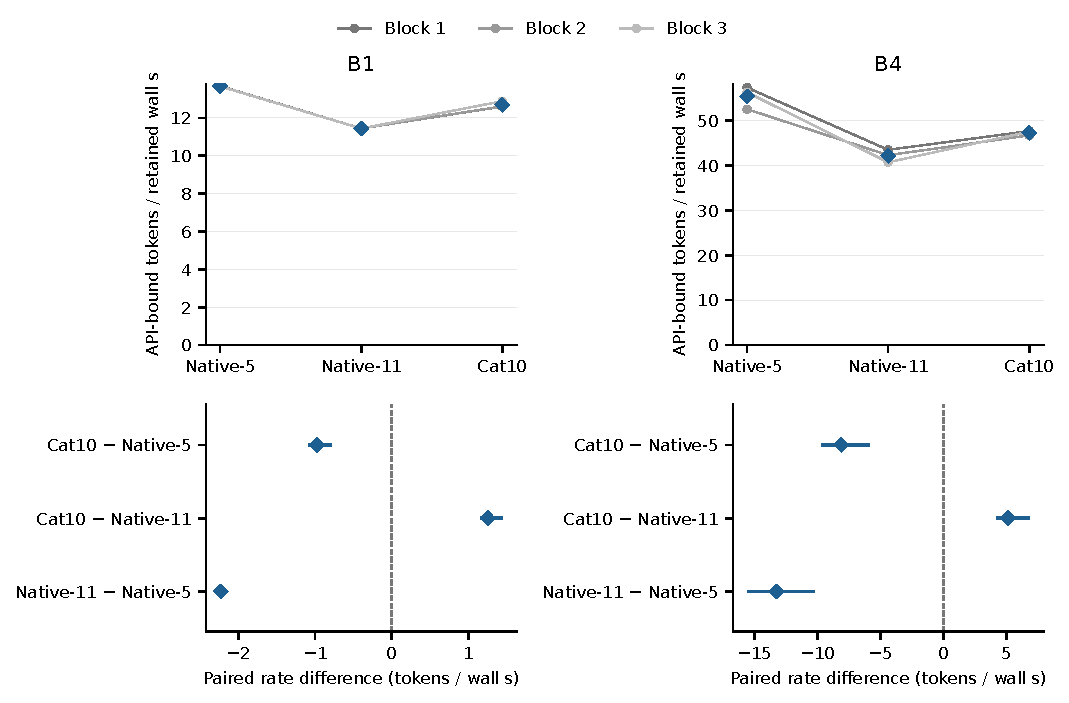
\includegraphics[width=0.94\textwidth]{figures/e1-timing.pdf}
\caption{E1: all eighteen initial fresh-boot cells on the pinned stack. Top: each gray line connects one paired block; blue diamonds mark the mean of three boot rates. Bottom: mean paired differences and the frozen 95\% bootstrap percentile intervals, resampling whole blocks separately at B1 and B4. Rates bind returned API tokens to unique retained wall intervals. These are as-executed instrumented configurations with different attention backends, the disclosed engine-seed deviation, and observed output divergence; they do not isolate a causal tree-algorithm effect.}
\label{fig:e1-timing}
\end{figure*}

\paragraph{Observed continuation divergence}
A retrospective comparison uses the complete timed API-ID streams, not just rate-support tokens. Across the three pairs of arms, three blocks, two batch conditions, and eight prompts, only 14 of 144 same-block prompt-stream pairs are exactly equal. Comparing the three block pairs within each arm/batch gives 72 equal pairs out of 144. Both native B1 arms repeat exactly in all 24 within-arm comparisons apiece; tree B1 does so in 8/24. At B4 the equality counts are 7/24 for MTP-5, 5/24 for MTP-11, and 4/24 for cat10. These dependent pair counts describe the observed streams, not an estimated population failure probability. They neither identify the source of divergence nor establish full-model sequential equivalence. Together with the seed and backend differences, they limit the result to measured output rates of the tested configurations on fixed input prefixes. No matched-continuation, quality-preservation, or isolated algorithm-speedup claim follows. The retrospective diagnostic does not alter the frozen eligibility, rates, intervals, or precision decisions.

\section{Limitations and Deferred Validation}
\label{sec:planned}
The archived and fresh measurements cover specific implementation stages, one main checkpoint family, and a limited task subset. The state contract is more general than its test coverage. Native-reference numerical agreement, sampler-law correctness, and deployment quality must remain separate claims. Instrumentation also has limits: H3 combines global structural-token counts with a pure-decode wall subset, so its proxy cannot establish matched decode or full-service throughput.

Table~\ref{tab:planned} lists the selected validation scope and deferred extensions. After configuration reconciliation (P0), three core experiments compare arithmetic on identical inputs (E7a), test numerical propagation and accepted-prefix continuation (E2/E7b), and measure the frozen implementation against strong chains (E1). E3 is conditional on promoting unfinished optimizations. E7a has completed kernel measurements, including fresh pilot and confirmation operands. E2/E7b supplies the bounded diagnostic and selected-route evidence above. E1 adds the eighteen-cell as-executed comparison above; its capture pilots and untimed preflights are not additional timing cells.

\begin{table*}[t]
\caption{Selected scope. Core experiments are E7a, E2/E7b, and E1, preceded by P0; E3 is conditional and other entries deferred. E7a, bounded E2/E7b checks, and the eighteen E1 cells are executed with their stated limits.}
\label{tab:planned}
\centering\footnotesize
\begin{tabularx}{\textwidth}{@{}p{0.08\textwidth}p{0.22\textwidth}Y>{\raggedright\arraybackslash}p{0.20\textwidth}@{}}
\toprule
ID & Question & Minimum comparison & Claim enabled \\
\midrule
P0 & What actually ran? & Archived binary, flags, sampling and denominator reconciliation & Correct configuration labels \\
E1 & Does the final tree beat strong chains? & Cat10, depth-comparable chain-5, longer chain-11; actual B1/B4; paired independent boots & As-executed decode-interval rates \\
E7a & Do arithmetic realizations agree? & Same operands: sequential, triangular solve, finite-Neumann; output and commit isolated & Numerical and local-cost characterization \\
E2/E7b & Do errors amplify or corrupt continuation? & Fixed-prefix stage substitutions; layer/final logits; state/KV/conv, sampler and cache fixtures & Scoped continuation and implementation agreement \\
E3 & Do optimizations combine? & Conditional scan/accept-walk toggles, individually and together & Composed local speedup \\
E4 & How does memory affect service latency? & Deferred: identical arrival trace and cache-capacity controls & Serving and cache explanation \\
E5 & Is broader task quality preserved? & Deferred: held-out tasks and powered quality design; exact sampler checks stay in E2 & Broader quality evidence \\
E6 & Does the result extend to NVFP4? & Deferred: matched native control and repeated composed tests & Quantization extension \\
E7c & How do authors' systems compare? & Deferred: feasible matched external implementations & Competitive system comparison \\
\bottomrule
\end{tabularx}
\end{table*}

E7a compares local reimplementations of published mechanisms, not the authors' systems. Identical captured operands and chosen paths isolate solver error from commit error. High-precision recurrence and each pinned native GPU path serve distinct reference roles. Its kernel-level pilot, the verified eight-prefix fresh-operand pilot, and the 32-prefix confirmation set evaluated against the record frozen from that pilot are reported in Section~\ref{sec:e7a-pilot}, including all identified frozen-rule failures and the retrospective audit of omitted checks. Those sample counts belong to E7a. Neither compact candidate met the frozen local criteria, so neither is promoted to an integrated serving or performance claim. E7b instead reports the bounded, single-prefix verifier-only and commit-only diagnostics and the offline fixed-input continuation in Section~\ref{sec:e7b-diagnostic}. The matched input-aligned windows are observed controls, not a general forced-path facility: the served route refuses the older forced-spine diagnostic. No combined-candidate confirmation campaign or powered task-quality study has been completed. Broader promotion would require those separate verification, commitment, combined-route, and continuation checks; the present failures remain reportable numerical findings.

E1 supplies controlled-prefix replay evidence for the tested instrumented configurations (Section~\ref{sec:e1-timing}). Its fixed-input prefixes produce different continuations, and the engine-seed mismatch prevents a fully controlled-settings interpretation. Matching numerator and denominator support fixes an accounting problem; it does not establish equivalent outputs, quality, or full-service latency. All eighteen initial cells are retained, and all six contrasts meet the prespecified precision target under coarse three-block resampling. Compact-route performance remains deferred because its numerical promotion criteria failed.

E2 combines existing analytic multidraft identities, multistep sampling tests, biased-selector controls, and accepted-path state fixtures~\cite{lumo2026archive} with the source-bound and actual-route checks in Section~\ref{sec:selected-route}. Graph execution, prefix-cache hits, stochastic deployment, and a full-model sequential oracle remain outside this finite qualification. Source availability alone is not a passing execution record, and historical numerical or garble checks do not prove distribution preservation.

\section{Conclusion}
\sys{} studies the implementation boundary between tree verification and the next native serving iteration. A correct continuation requires agreement among recurrent state, convolution history, attention KV, physical row mappings, and the sampler. The archived failures show that satisfying one surface can leave another inconsistent.

The KV-remap fixture improved from 15/15 failures to 0/15, and the numerical investigation produced a shared-spine repair with byte agreement in its tested checks (Table~\ref{tab:correctness}). In the later three-arm campaign, the tree's archived structural-token/pure-wall proxy was 32.85 versus native MTP-5's 42.74 (Table~\ref{tab:three-arm}). The underlying event populations differ, so those values preserve an accounting observation rather than establish a measured throughput ranking. A separate paired attention optimization reduced its tested B4 step by 27.03\,ms (Table~\ref{tab:optimization})~\cite{lumo2026archive}.

These findings support a scoped account of state integrity, numerical execution, and serving cost. They do not establish superiority over direct GDN tree methods or a distribution-preservation guarantee for the current implementation. Configuration reconciliation has documented unresolved historical binary identity and duplicated sampling constraints. Fresh same-input arithmetic and selected-route B1/B4 checks add bounded numerical and continuation evidence. Eighteen current-stack boots bind API outputs to retained decode wall intervals: the tree averages 12.69 versus native MTP-5's 13.67 tokens/s at B1, and 47.28 versus 55.38 at B4, while exceeding MTP-11. Different generated continuations, attention backends, and engine seeds constrain that result to the configurations as executed.

\label{ReferencesStart}
\bibliographystyle{IEEEtran}
\bibliography{ref}
\end{document}
